\chapter{Implementación}

\section{Datos}
Los datos han sido recolectados de la página oficial de Sofascore \cite{Sofascore} mediante scrapeo. Para ver las estadísticas de un partido desde la página, basta con irse a ese partido y a 'Estadísticas del jugador' donde se mostrarán todos los jugadores que jugaron el partido. El mapa de calor lo obtengo a través de una API que tiene una función predefinida para eso. 

Para poder meter los datos de un partido hay que escribir el nombre del jugador, equipo, rival que se desea almacenar y la url de ese partido y automáticamente se meterán sus datos en la base de datos.

El código son más de cien líneas y la mayoría son ajustes del scrapeo, por lo que se ha considerado no ponerlo aquí, pero se puede ver directamente en GitHub.

\subsection{Mapas de calor}
Las estadísticas de los jugadores se almacenan como enteros o flotantes y muestran simplemente el valor de dicha estadística (por ejemplo, pases clave, 7), sin embargo, los mapas de calor son diferentes. En cada uno se almacena una lista con una pareja de enteros que representan las coordenadas x e y en el campo. 

Para representar el campo de fútbol se ha hecho uso de las librerías matplotlib y mplsoccer para su representación, esta última es la que permite dibujar el campo. El código para representar un campo vacío sería este:

\begin{lstlisting}[language=Python, caption={Representación campo vacío}, label={lst:codigo-python}]
import matplotlib.pyplot as plt
from mplsoccer import Pitch

fig, ax = plt.subplots(figsize=(16, 9))
pitch = Pitch(pitch_type='opta')
pitch.draw(ax=ax)
plt.show()
\end{lstlisting}

La representación del campo vacío quedaría:

\begin{figure}[H]
    \centering
    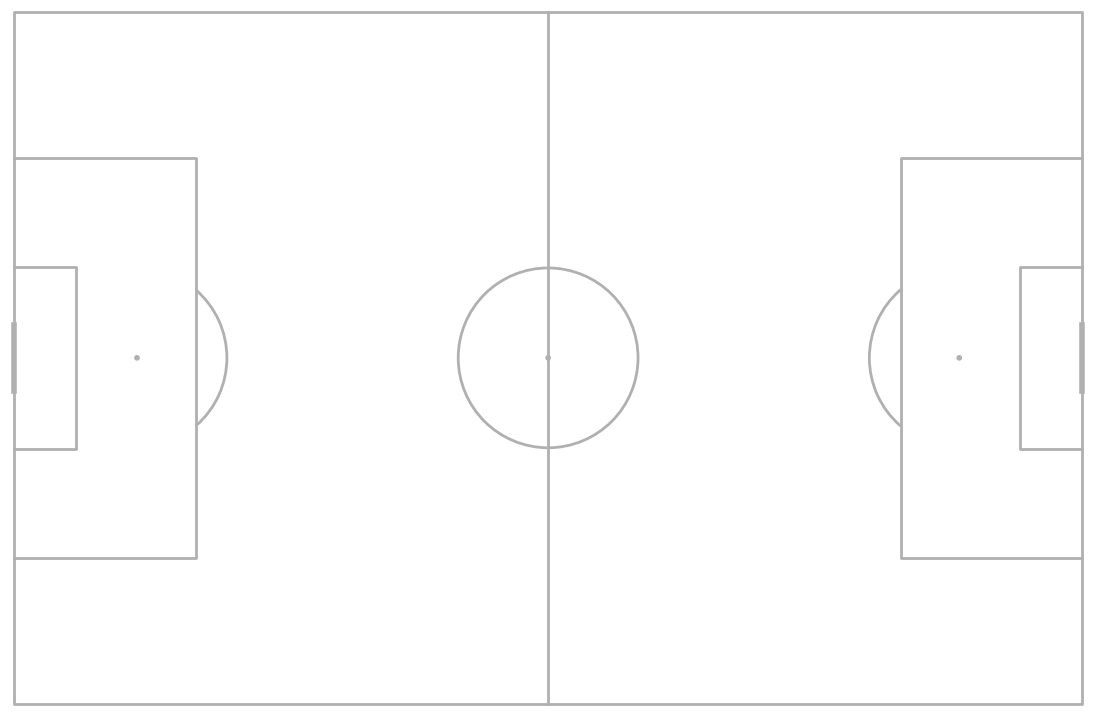
\includegraphics[width=0.7\textwidth]{plantilla-TFG-ETSIIT/doc/imagenes/Campo_vacio.png}
    \caption{Reprentación campo de fútbol}
    \label{fig:etiqueta-imagen}
\end{figure}

Es importante recalcar que el punto (0, 0) está abajo a la izquierda y el (99, 99) arriba a la derecha, por lo que los mapas siempre se verán de izquierda a derecha, incluso cuando el jugador juegue de visitante se ajustarán sus datos para que se vea de la misma manera siempre y no dejar lugar a dudas.

Para representar el mapa de un jugador concreto solo tenemos que obtenerlo de su base de datos y representarlo de la misma manera que antes, pero rellenando el campo con sus puntos, el código es el siguiente:

\begin{lstlisting}[language=Python, caption={Mapa de calor de un futbolista}, label={lst:codigo-python}]

from pymongo import MongoClient
import pandas as pd
import matplotlib.pyplot as plt
from mplsoccer import Pitch
import warnings
from matplotlib.colors import LinearSegmentedColormap

warnings.filterwarnings("ignore")

# Conexion a mongoDB
cliente = MongoClient("mongodb://localhost:27017")
db = cliente["TFG"]
coleccion_jugadores = db["jugadores"]

# Buscar un jugador
jugador = coleccion_jugadores.find_one({"nombre": "Luis Milla", "equipo": "Getafe", "rival": "Villareal"})

# Verificar si se encontro el jugador
if jugador:

    mapa_calor_lista = jugador["mapa_calor"]
    mapa_calor_df = pd.DataFrame(mapa_calor_lista)
    colors = [(0, "white"), (0.5, "orange"), (1, "red")]
    custom_cmap = LinearSegmentedColormap.from_list("custom_cmap", colors)

    fig, ax = plt.subplots(figsize=(16, 9))

    pitch = Pitch(pitch_type='opta')
    pitch.draw(ax=ax)
    pitch.kdeplot(mapa_calor_df.x, mapa_calor_df.y, ax=ax,
                fill = True,
                levels=100,
                thresh=0.08,
                zorder=-1,
                bw_adjust=0.15,
                cmap="OrRd")

    # Anadir titulo personalizado
    nombre = jugador["nombre"]
    equipo = jugador["equipo"]
    rival = jugador["rival"]
    plt.title(f"Mapa de calor del jugador \"{nombre}\" del equipo \"{equipo}\", rival \"{rival}\"", fontsize=18)

    plt.show() 

else:
    print("Jugador no encontrado.")

\end{lstlisting}

Los ajustes de los valores de representación del mapa se han hecho a mano dejando los que se consideraban más adecuados para la visualización del mapa de calor. Vamos a ejemplificarlo con algunos jugadores.

El jugador Luis Milla del Getafe es centrocampista y su mapa de calor en el partido contra el Villarreal de liga de la temporada 2024/2025 se ve de la siguiente manera:

\begin{figure}[H]
    \centering
    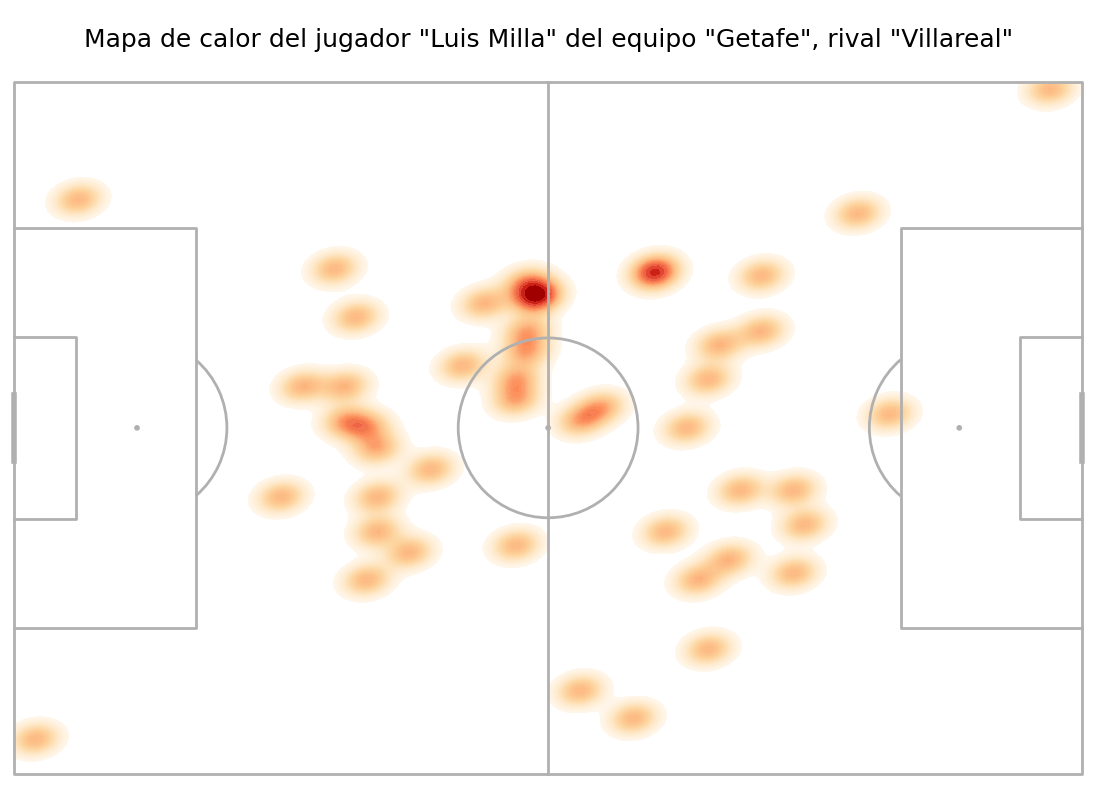
\includegraphics[width=0.7\textwidth]{plantilla-TFG-ETSIIT/doc/imagenes/Mapa_MC.png}
    \caption{Ejemplo representación de MC}
    \label{fig:etiqueta-imagen}
\end{figure}

Vamos a ver más ejemplos de otras posiciones distintas. El de un lateral derecho se vería algo parecido a esto:

\begin{figure}[H]
    \centering
    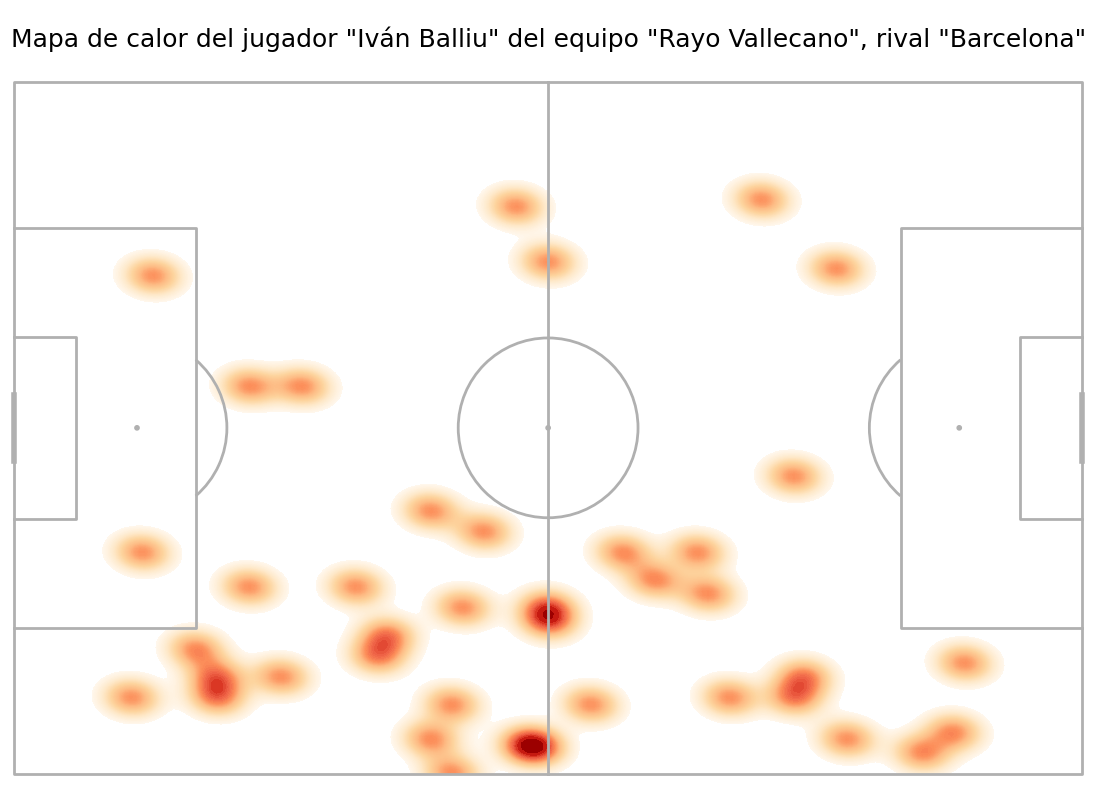
\includegraphics[width=0.7\textwidth]{plantilla-TFG-ETSIIT/doc/imagenes/Mapa_LD.png}
    \caption{Ejemplo representación de LD}
    \label{fig:etiqueta-imagen}
\end{figure}

Como se puede apreciar, al ser un lateral derecho tiene predominancia en la parte de abajo del campo ya que recordemos se ve izquierda a derecha y de abajo a arriba.

Un ejemplo de un delantero extremo izquierdo se vería algo así:

\begin{figure}[H]
    \centering
    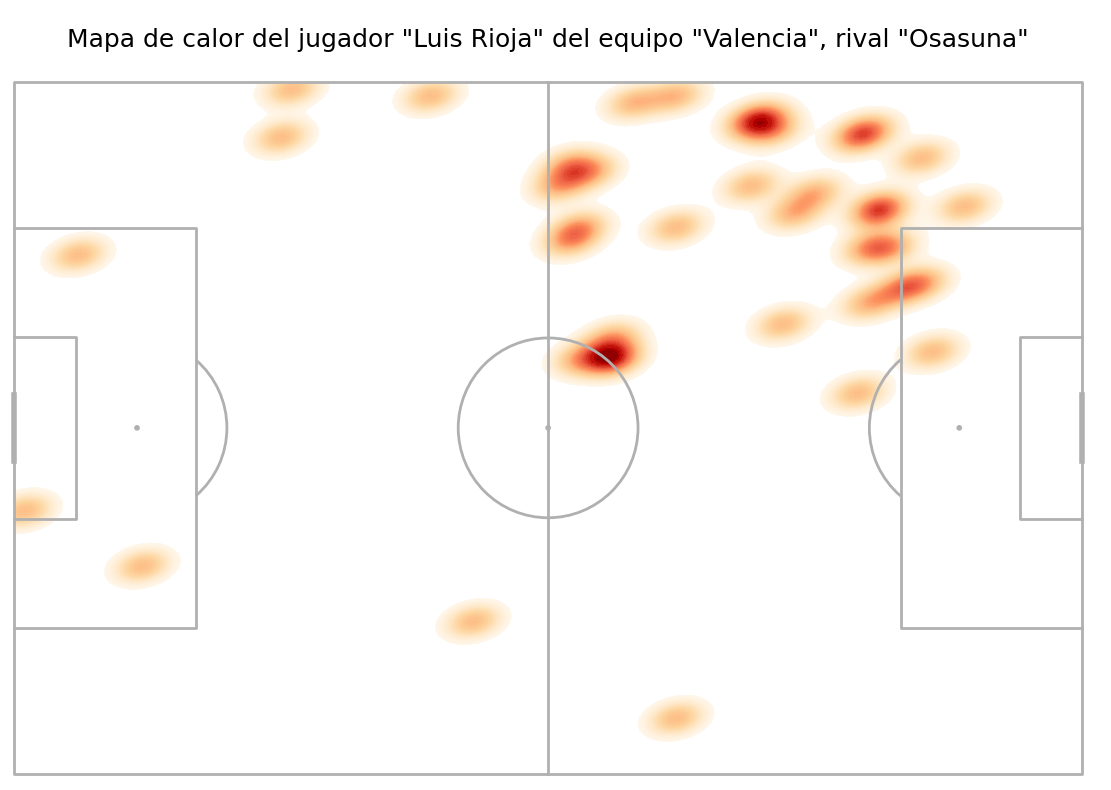
\includegraphics[width=0.7\textwidth]{plantilla-TFG-ETSIIT/doc/imagenes/Mapa_EI.png}
    \caption{Ejemplo representación de EI}
    \label{fig:etiqueta-imagen}
\end{figure}

Como se ve en la imagen, predomina principalmente la zona de arriba a la derecha que es la que pertenece al extremo izquierdo.

Por último, vamos a ver el mapa de calor de un portero, al que rara vez vamos a ver fuera del área.

\begin{figure}[H]
    \centering
    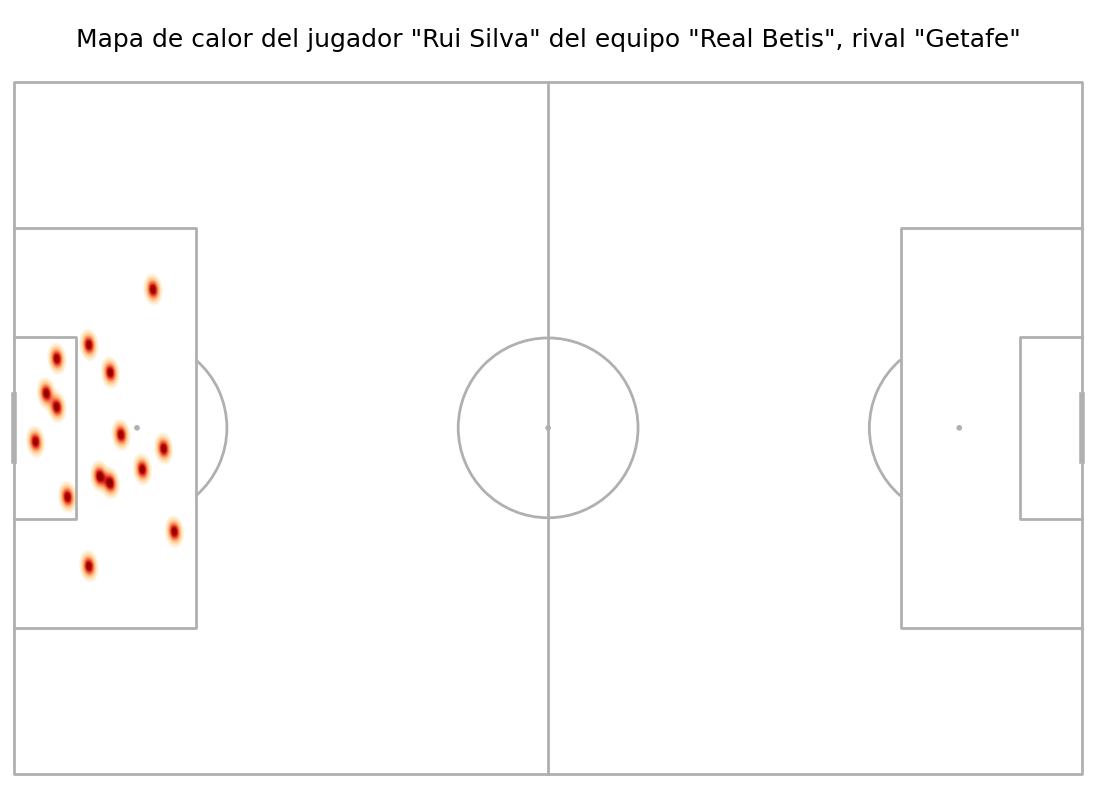
\includegraphics[width=0.7\textwidth]{plantilla-TFG-ETSIIT/doc/imagenes/Mapa_POR.png}
    \caption{Ejemplo representación de POR}
    \label{fig:etiqueta-imagen}
\end{figure}

También es importante recalcar que los mapas de calor pueden ser algo aleatorios, aunque los jugadores suelen respetar bastante su posición, en los partidos ocurren eventos inesperados y puede que haya influido en otras zonas, aunque son casos aislados. Por ejemplo, en el caso del extremo izquierdo tocó el balón 3 veces en su área, algo que no es habitual por lo que se puede suponer que quizá sea por defender jugadas a balón parado. O el primero que hemos visto, Luis Milla, que es centrocampista toca el balón en las 2 esquinas del campo por lo que se intuye que ha sido para sacar los córneres.

\section{Algoritmo sin zonas}

Una vez obtenidos los datos de los jugadores en la base de datos se va a pasar a explicar la implemetación del algoritmo sin zonas, en decir, solo teniendo en cuenta las estadísticas de los futbolistas y sin dividir el campo en zonas. No se ha considerado poner todas las funciones porque son demasiadas, pero sí la función principal del programa que es la siguiente:

\begin{lstlisting}[language=Python, caption={Algoritmo sin zonas}, label={lst:codigo-python}]
if not JUGADORES_CACHE:
    inicializar_cache_jugadores()
#Bucle que recorre todos los partidos
for partido in coleccion_partidos.find():
    # Obtener jugadores
    jugadores1 = [jug for jug in JUGADORES_CACHE.values() if jug["equipo"] == partido["Local"] and jug["rival"] == partido["Visitante"] and jug["temporada"] == partido["Temporada"]]
    jugadores2 = [jug for jug in JUGADORES_CACHE.values() if jug["equipo"] == partido["Visitante"] and jug["rival"] == partido["Local"] and jug["temporada"] == partido["Temporada"]]
    
    maximos = calcularMaximos(jugadores1, jugadores2)

    suma_total_ofensiva_e1 = 0
    suma_total_defensiva_e1 = 0
    suma_total_ofensiva_e2 = 0
    suma_total_defensiva_e2 = 0

    for j in jugadores1:
        estadisticas_ofensivas = getEstadisticasOfensivas(j["_id"], maximos)
        estadisticas_defensivas = getEstadisticasDefensivas(j["_id"], maximos)
        suma_total_ofensiva_e1 += estadisticas_ofensivas
        suma_total_defensiva_e1 += estadisticas_defensivas
    for j in jugadores2:
        estadisticas_ofensivas = getEstadisticasOfensivas(j["_id"], maximos)
        estadisticas_defensivas = getEstadisticasDefensivas(j["_id"], maximos)
        suma_total_ofensiva_e2 += estadisticas_ofensivas
        suma_total_defensiva_e2 += estadisticas_defensivas
    
    total_e1 = suma_total_ofensiva_e1 - suma_total_defensiva_e2
    total_e2 = suma_total_ofensiva_e2 - suma_total_defensiva_e1

    resultado = total_e1 - total_e2

    if resultado > 2:
        resultado = "local"
    elif resultado < -2:
        resultado = "visitante"
    else:
        resultado = "empate"
\end{lstlisting}

Como se describió antes, es solo la sumatoria de las estadísticas normalizadas de todos los jugadores del equipo. El equipo que saque más puntuación gana. Como se puede observar, el valor que determina dónde cortar para elegir es 2, al ser un programa simple donde no se ha utilizado ninguna técnica de marchine learning se ha puesto a mano.

Las funciones getEstadisticasOfensivas y getEstadisticasDefensivas recorren los datos del jugador y se quedan con las estadísticas correspondientes normalizadas entre 0 y 1, siendo 1 la máxima ejecución de esa estadística en el partido y 0 la menor.

\begin{figure}[H]
    \centering
    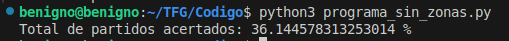
\includegraphics[width=1.0\textwidth]{plantilla-TFG-ETSIIT/doc/imagenes/Ejecucion_simple.png}
    \caption{Ejecución algoritmo sin zonas}
    \label{fig:etiqueta-imagen}
\end{figure}

Ejecutando todos los partidos de la base de datos sale una precisión del 36.14\%, algo que se puede considerar bajo ya que solo hay 3 resultados posibles de un partido: gana local, gana visitante o empate; por lo que esta predicción es casi lo mismo que hacerlo al azar ya que cada uno tiene una probabilidad de un 33\% de salir.

\section{Algoritmo con pesos}
Se va a proceder a implementar el algoritmo explicado en la sección anterior. Como se indicó, se ha decidido dividir el terreno de juego en 24 zonas y cada una tendrá un peso. La división del campo en zonas es la siguiente:

\begin{figure}[H]
    \centering
    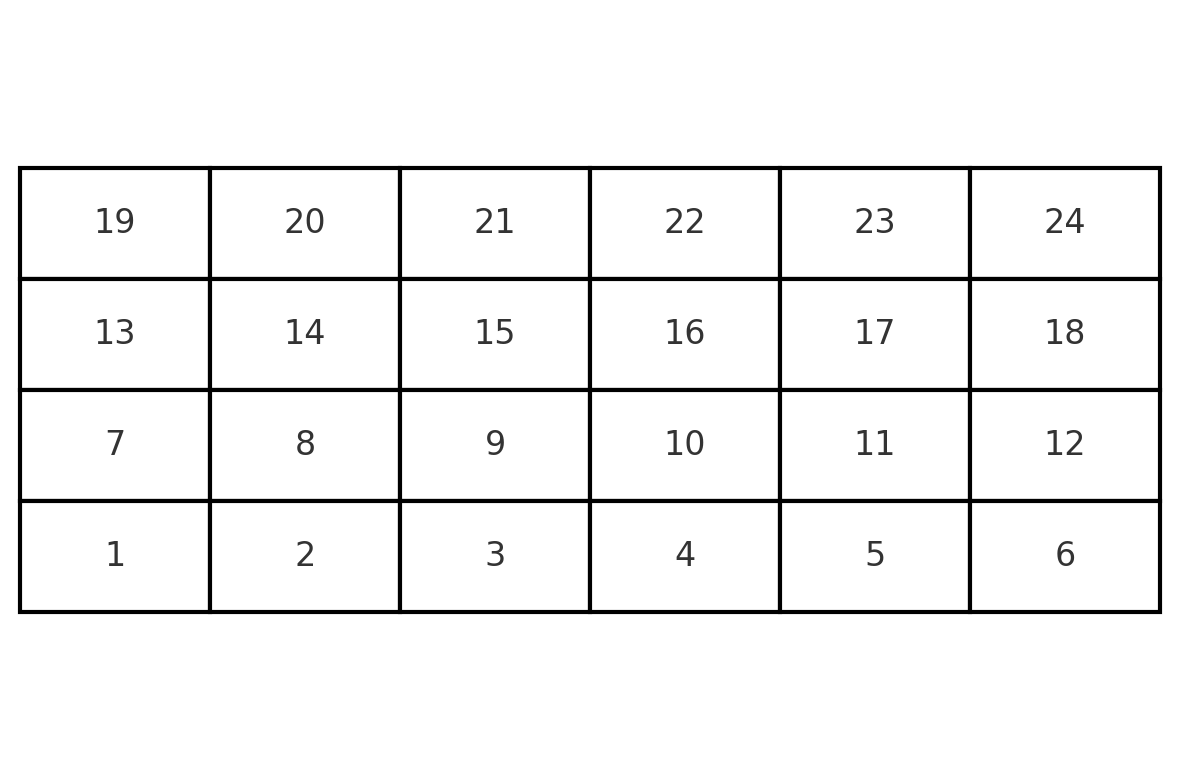
\includegraphics[width=0.8\textwidth]{plantilla-TFG-ETSIIT/doc/imagenes/Zonas_campo.png}
    \caption{Distribución en zonas del campo}
    \label{fig:etiqueta-imagen}
\end{figure}

Al igual que antes, el campo se ve de izquierda a derecha, siendo las zonas 6, 12, 18 y 24 las de máximo ataque y 1, 7, 13, 19 las más defensivas.

Para este problema inicial se ha implementado 2 vectores de pesos, uno para las estadísticas constructivas (de ataque) y otro para las destructivas (de defensa), aunque en el código se ha tratado como un único vector realmente.

La separación de vectores se hace para evaluar correctamente a cada estadística, pues no tendría sentido ponderar las acciones defensivas con un peso bajo al no ser una zona de ataque. El vector de ataque va aumentando gradualmente conforme las zonas se acercan al área rival y el vector de defensa al contrario, va aumentando conforme te acercas a tu propia portería.

De esta manera obtenemos los 2 vectores siguientes. El vector inicial para las estadísticas ofensivas:

\begin{figure}[H]
    \centering
    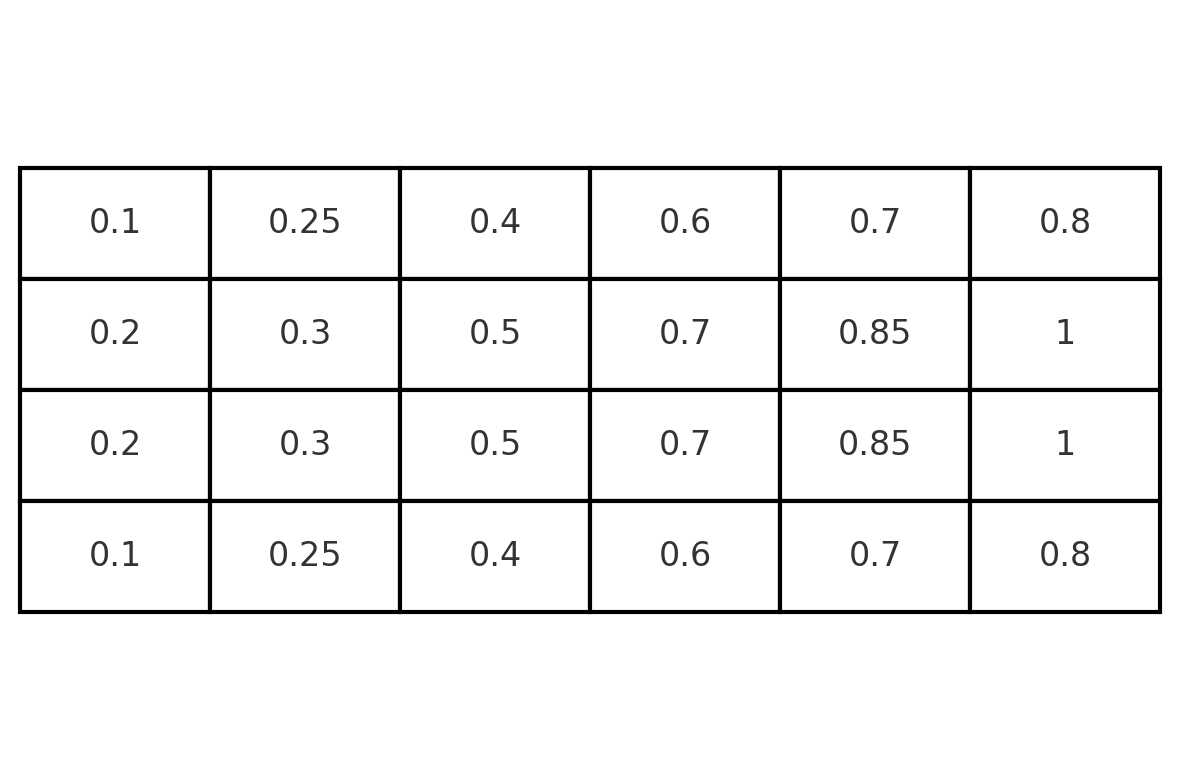
\includegraphics[width=0.8\textwidth]{plantilla-TFG-ETSIIT/doc/imagenes/Pesos_ini_ataque.png}
    \caption{Vector inicial de ataque}
    \label{fig:etiqueta-imagen}
\end{figure}

Y el vector inicial para las estadísticas defensivas:

\begin{figure}[H]
    \centering
    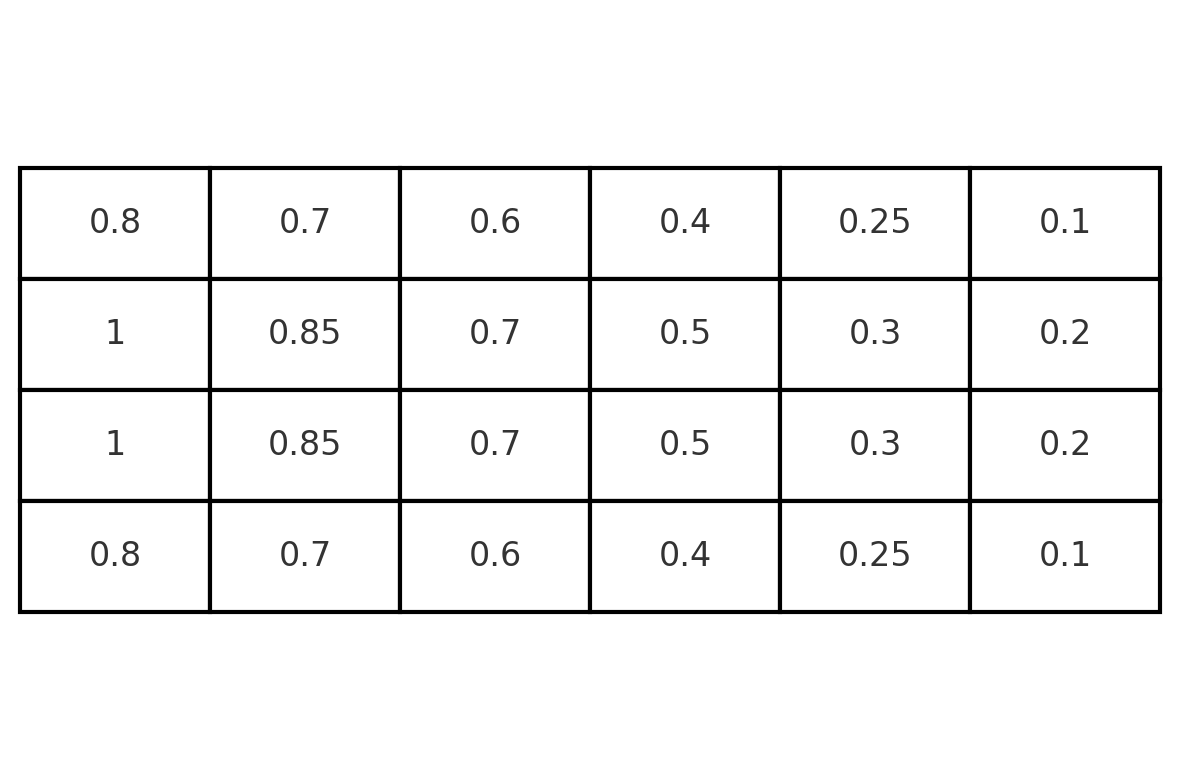
\includegraphics[width=0.8\textwidth]{plantilla-TFG-ETSIIT/doc/imagenes/Pesos_ini_defensa.png}
    \caption{Vector inicial de defensa}
    \label{fig:etiqueta-imagen}
\end{figure}

Una vez se han definido los pesos de cada zona se va a pasar a definir la implementación del algoritmo. Primero se tienen que inicializar los datos de los jugadores de ese partido.

\begin{lstlisting}[language=Python, caption={Inicialización datos}, label={lst:codigo-python}]
def calcula_zonas(local, visitante, temporada, corte=2):
    if not JUGADORES_CACHE:
        inicializar_cache_jugadores()

    # Obtener el partido
    partido = resultados.find_one({"Local": local, "Visitante": visitante, "Temporada": temporada})
    if not partido:
        raise ValueError(f"No se encontro el partido entre {local} y {visitante} en la temporada {temporada}.")

    jugadores1 = [jug for jug in JUGADORES_CACHE.values() if jug["equipo"] == local and jug["rival"] == visitante and jug["temporada"] == temporada]
    jugadores2 = [jug for jug in JUGADORES_CACHE.values() if jug["equipo"] == visitante and jug["rival"] == local and jug["temporada"] == temporada]
    
    preprocesar_mapa_calor(jugadores1)
    preprocesar_mapa_calor(jugadores2)

    maximos = calcularMaximos(jugadores1, jugadores2)

\end{lstlisting}

Primero se inicializan los jugadores en la caché, esto se hace para disminuir las consultas a la base de datos. De esta forma se buscan todos los jugadores una vez y se guardan en una variable llamada $\text{JUGADORES\_CACHE}$.

Después, se busca el partido con una consulta y se inicializan las variables con los jugadores deseados. Se procesan los mapas de calor, donde se calcula el porcentaje que ha estado el jugador en cada zona. Por último, se calculan los máximos que hay de cada estadística y se guarda en una variable local.

\begin{lstlisting}[language=Python, caption={Procesamiento de cada zona}, label={lst:codigo-python}]
for z in zonas[:-1]:
        suma_total_ofensiva_e1 = 0
        suma_total_defensiva_e1 = 0
        suma_total_ofensiva_e2 = 0
        suma_total_defensiva_e2 = 0
        for j in jugadores1:
            porc = calcularPorcentaje(j, z)
            if porc != 0:
                estadisticas_ofensivas = getEstadisticasOfensivas(j["_id"], maximos) * porc
                estadisticas_defensivas = getEstadisticasDefensivas(j["_id"], maximos) * porc
                suma_total_ofensiva_e1 += estadisticas_ofensivas
                suma_total_defensiva_e1 += estadisticas_defensivas

        for j2 in jugadores2:
            porc = calcularPorcentaje(j2, z)
            if porc != 0:
                estadisticas_ofensivas = getEstadisticasOfensivas(j2["_id"], maximos) * porc
                estadisticas_defensivas = getEstadisticasDefensivas(j2["_id"], maximos) * porc
                suma_total_ofensiva_e2 += estadisticas_ofensivas
                suma_total_defensiva_e2 += estadisticas_defensivas

\end{lstlisting}

El código hace lo siguiente, por cada zona del campo se recorren los jugadores de ambos equipos, por cada jugador de cada equipo se extraen sus estadísticas y se multiplican por el porcentaje de influencia del jugador en esa zona según el mapa de calor. Las estadísticas ya están normalizadas y se añaden directamente al total de su equipo.

\begin{lstlisting}[language=Python, caption={Procesamiento de cada zona}, label={lst:codigo-python}]
    zonas_valores_e1[z-1] = (suma_total_ofensiva_e1*zonas_coeficientes[z-1] - suma_total_defensiva_e2*zonas_coeficientes[z-1+24])
    
    zonas_valores_e2[z-1] = (suma_total_ofensiva_e2*zonas_coeficientes[z-1] - suma_total_defensiva_e1*zonas_coeficientes[z-1+24])
    
    total_rival[z-1] = (suma_total_ofensiva_e2*zonas_coeficientes[z-1] + suma_total_defensiva_e1*zonas_coeficientes[z-1+24])

suma_total = sum(zonas_valores_e1) - sum(zonas_valores_e2)

if suma_total > corte:
    return 1
elif suma_total < -corte:
    return 2
else:
    return 0

\end{lstlisting}

Una vez obtenidos el total ofensivo y defensivo de cada equipo solo queda multiplicarlo por el peso que tenga cada zona y compararlos, según el número resultante gana uno, otro o empatan.

\begin{figure}[H]
    \centering
    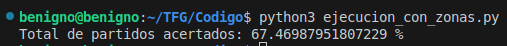
\includegraphics[width=1.0\textwidth]{plantilla-TFG-ETSIIT/doc/imagenes/Ejecucion_con_zonas.png}
    \caption{Ejecución algoritmo con zonas}
    \label{fig:etiqueta-imagen}
\end{figure}

Si ejecutamos todos los partidos de la base de datos con este algoritmo, obtenemos una precisión del 67.47\%, algo que ya es mucho más aceptable que antes, aunque todavía se puede mejorar más.

Una funcionalidad extra que tiene el algoritmo es que, gracias a que calcula la sumatoria total en cada zona de los 2 equipos, podemos ver qué equipos han dominado en cada zona. Esto se hace gracias a la función 'representar\_mapa', a la que se le pasan 2 argumentos que son los 2 vectores con la sumatoria total de cada equipo en cada zona del campo, de esta manera crea un mapa de 24 zonas y colorea en rojo las zonas en las que domina el equipo 1 y en azul las que domina el equipo 2. También se tienen en cuenta la simetría de los equipos, para que se siga viendo igual que hasta ahora de izquierda a derecha se ajustan las estadísticas del visitante para que también ataque de izquierda a derecha. Por lo que si el visitante domina en ataque lo veremos en la zona en la que nosotros vemos siempre el ataque, solo que de color azul porque es el visitante.

Un ejemplo de este mapa en el Villarreal - Las Palmas de la liga española temporada 2024/2025:

\begin{figure}[H]
    \centering
    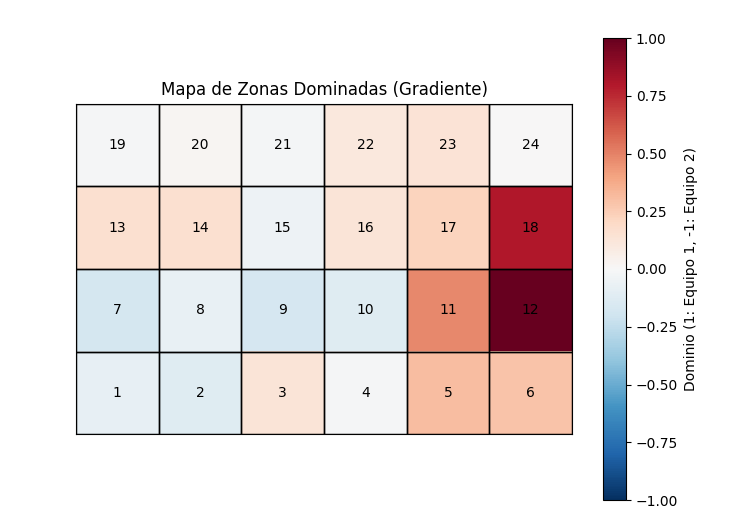
\includegraphics[width=0.7\textwidth]{plantilla-TFG-ETSIIT/doc/imagenes/Local_zonas_equipos.png}
    \caption{Mapa de zonas resultante del Villareal - Las Palmas}
    \label{fig:etiqueta-imagen}
\end{figure}

Como se puede apreciar el equipo local, el Villarreal, dominó totalmente las zonas de ataque, especialmente las más cerca de la portería rival, esto tiene sentido pues el Villarreal ganó este partido 3-1. De esta manera un entrenador podría sacar conclusiones sobre el partido y ver qué zonas debería mejorar, por ejemplo el equipo visitante ha recibido más ataques sobre la banda derecha, llegando incluso a línea de fondo, por lo que tendría que defender más esa zona. El entrenador del Villarreal podría llegar a la conclusión de que fue un partido muy bueno de su equipo ya que practicamente no perdieron en ninguna zona, o si lo hacen es por muy poco pudiendo considerarse casi un empate.

Vamos a ver ahora un ejemplo donde gana el equipo visitante:

\begin{figure}[H]
    \centering
    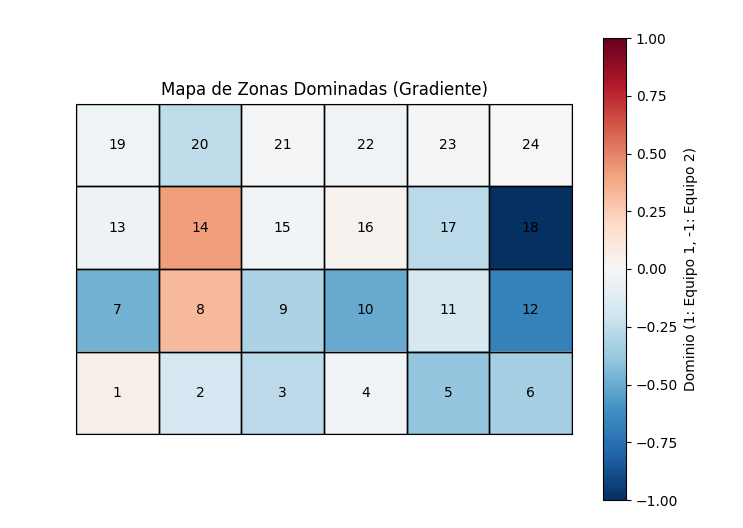
\includegraphics[width=0.7\textwidth]{plantilla-TFG-ETSIIT/doc/imagenes/Visitante_zonas_equipo.png}
    \caption{Mapa de zonas resultante del Getafe - Las Palmas}
    \label{fig:etiqueta-imagen}
\end{figure}

Como se puede apreciar, el equipo visitante, que representa de color azul, ha dominado en prácticamente en todas las zonas del campo, menos en las 2 zonas principales de defensa. Lo que puede llevar a la conclusión de que el equipo local se dedicó principalmente a defender, concentrando sus acciones defensivas en esas zonas, pero a pesar de sus esfuerzos no logró parar el vendaval ofensivo del rival.

Ahora vamos a ver uno en el que los 2 equipos empaten:
\begin{figure}[H]
    \centering
    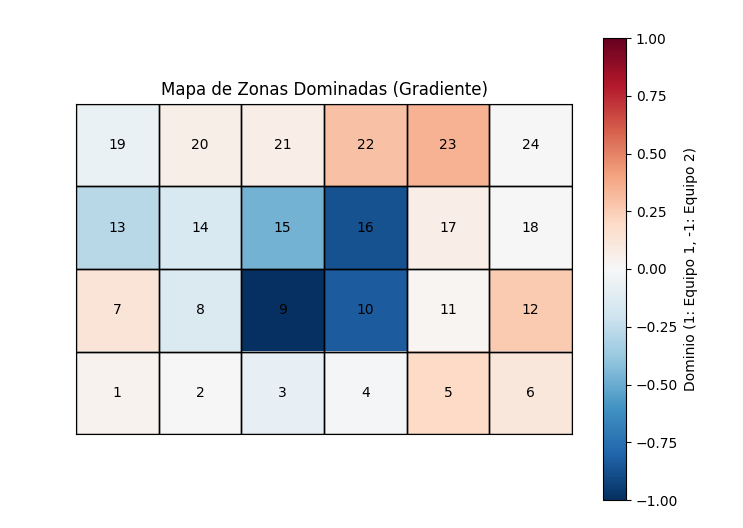
\includegraphics[width=0.7\textwidth]{plantilla-TFG-ETSIIT/doc/imagenes/Empate_zonas_equipos.png}
    \caption{Mapa de zonas resultante del Las Palmas - Sevilla}
    \label{fig:etiqueta-imagen}
\end{figure}

En este ejemplo entre Las Palmas - Sevilla de la liga española de la temporada 2024/2025, ningún equipo consiguió dominar el área rival, sin embargo, el centro del campo sí fue dominado por el local, aunque esto no le sirvió para la victoria.

Esta información puede serle muy útil a los entrenadores ya que pueden ver en qué zonas el equipo debe mejorar y sacar conclusiones del resultado del partido.

\section{Rendimiento individual de cada futbolista}
En el fútbol, no solo es importante analizar al equipo, sino que también lo es hacerlo para cada jugador individualmente. De la misma manera que se pueden acceder a las características totales almacenadas por el equipo en cada zona, también se puede hacer para cada jugador individualmente. Esto nos puede servir para ver qué jugadores son los que han aportado menos en el partido o cuáles han sido los más desequilibrantes.

La manera de valorarlos es la siguiente, si la sumatoria de estadísticas de un rival en una zona es mayor o ligeramente inferior que la suma total del equipo rival en esa zona es porque el futbolista ha sido diferencial.
Vamos a ver algunos mapas de calor de unas futbolistas de la liga F al aplicar esto en el partido
Real Madrid F - Valencia F:

\begin{figure}[H]
    \centering
    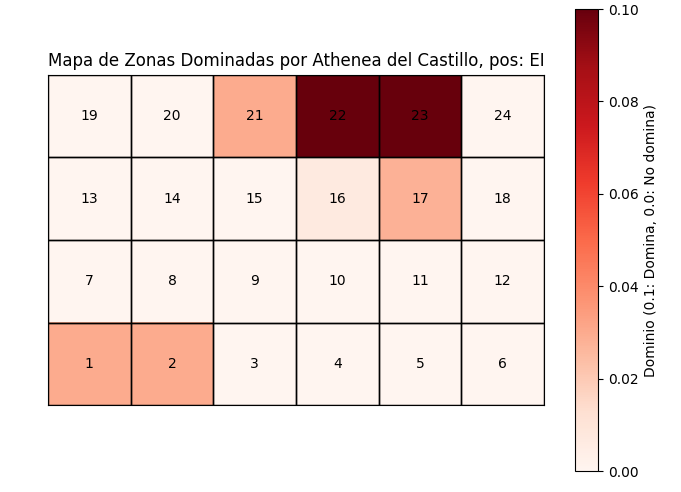
\includegraphics[width=0.7\textwidth]{plantilla-TFG-ETSIIT/doc/imagenes/futbolista_mapa_1.png}
    \caption{Mapa de influencia de Athenea de Castillo}
    \label{fig:etiqueta-imagen}
\end{figure}

Este mapa indica que las zonas que hay coloreadas son los sitios donde la jugadora ha sido superior a todo el equipo rival en cuanto a estadísticas. El rojo significa que ha sido superior y el azul que ha sido ligeramente inferior, las que no están coloreadas es porque ha sido claramente inferior. Como se puede apreciar, esta futbolista que es extrema izquierda fue muy diferencial en el partido ya que dominó las zonas de su posición.

Vamos a ver este otro mapa de una lateral derecha:

\begin{figure}[H]
    \centering
    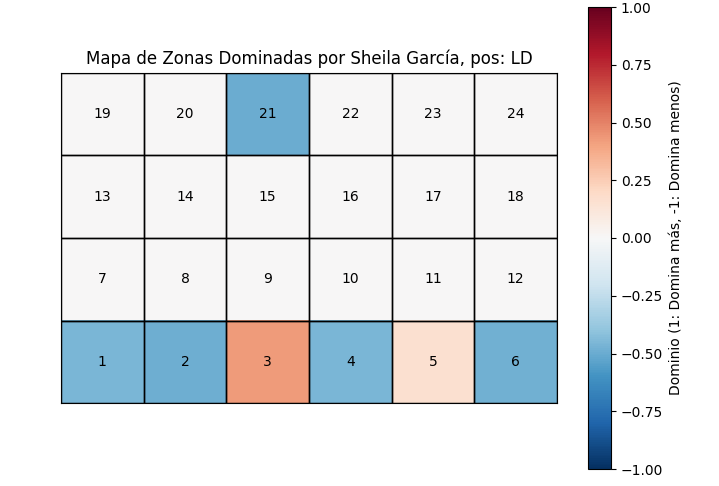
\includegraphics[width=0.7\textwidth]{plantilla-TFG-ETSIIT/doc/imagenes/Futbolista_mapa_2.png}
    \caption{Mapa de influencia de Sheila García}
    \label{fig:etiqueta-imagen}
\end{figure}

Como se puede ver en la imagen, esta futbolista fue claramente diferencial en su banda, algo que tiene sentido ya que fue valorada como una de las mejores del partido.

Vamos a ver el mapa de la extrema izquierda que entró a sustituir a la que había:

\begin{figure}[H]
    \centering
    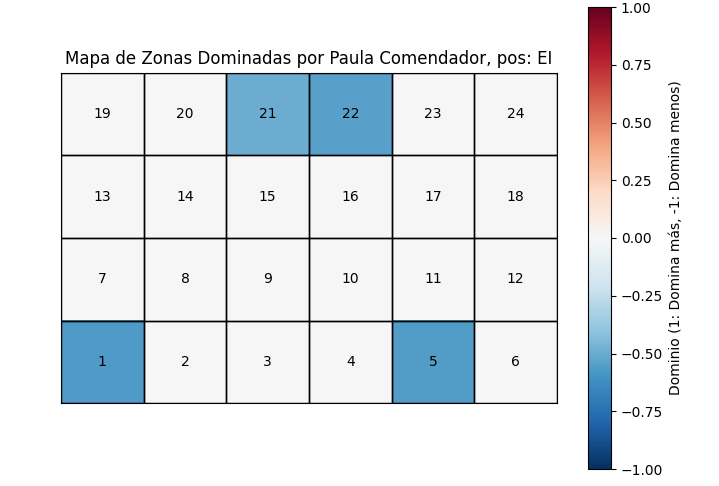
\includegraphics[width=0.7\textwidth]{plantilla-TFG-ETSIIT/doc/imagenes/Futbolista_mapa_3.png}
    \caption{Mapa de influencia de Paula Comendador}
    \label{fig:etiqueta-imagen}
\end{figure}

Como se puede ver, esta futbolista no fue tan diferencial en el partido como la otra extremo titular que se ha visto antes. Esto le puede servir al entrenador para tomar decisiones sobre las alineaciones.

Vamos a ver un último ejemplo con una defensa central del partido Barcelona F - Athletic Club de Bilbao F:

\begin{figure}[H]
    \centering
    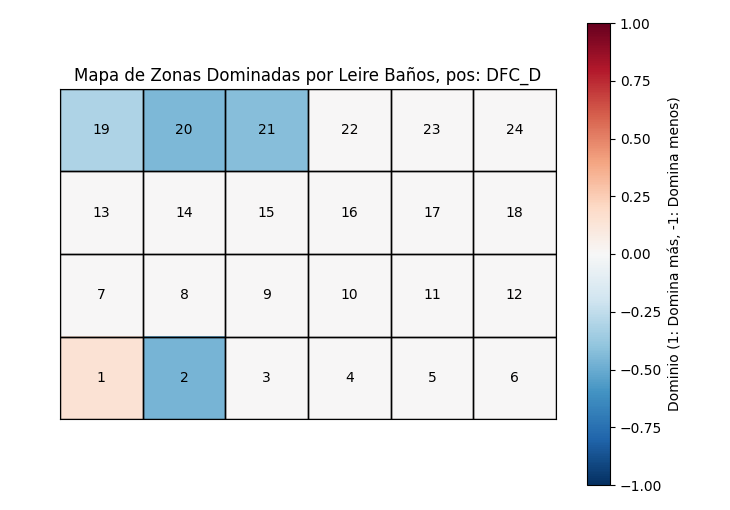
\includegraphics[width=0.7\textwidth]{plantilla-TFG-ETSIIT/doc/imagenes/futbolista_mapa_4.png}
    \caption{Mapa de influencia de Leire Baños}
    \label{fig:etiqueta-imagen}
\end{figure}

En este partido, se puede deducir que la central por la derecha hizo un mal partido ya que en las zonas del centro de la defensa no consigue ganar, solo un poco en los laterales, por lo que el entrenador podría deducir que la jugadora ha tenido que salir de su posición para llegar a las ayudas en defensa para las laterales.

Estas son interpretaciones que podría hacer un entrenador de fútbol, interpretando situaciones del juego como las coberturas, la presión alta o los juegos por las bandas, incluso podrían llegar a ser mucho más profundas interpretando el estilo de juego del rival. Es otra manera de ver cómo con esta técnica el entrenador puede llegar a preparar mejor un partido.

\section{Algoritmo genético}

Para implementarlo, definimos al vector de ataque y defensa como un único vector que será considerado como un miembro de la población. Tendrá un tamaño de 48, ya que hay que tener en cuenta las ponderaciones de ataque y de defensa, estas ponderaciones tendrán un valor entre 0 y 1.

\subsection*{Función de evaluación}
Para medir la calidad de un individuo se utiliza la función 'evaluar\_vector' a la que se le pasa como argumento el vector de coeficientes y lo ejecuta en todos los partidos de la base de datos, dando así el porcentaje de acierto que tiene ese vector. Cuanto mayor sea ese porcentaje de aciertos mayor será la calidad del individuo.

\subsection*{Operadores genéticos}

Para la selección se ha optado por una selección por torneo. En \cite{algoritmo_genetico}, podemos ver cómo de precisa es esta técnica, ya que mezcla aleatoriedad con la selección de los mejores individuos.

\begin{lstlisting}[language=Python, caption={Selección por torneo}, label={lst:codigo-python}]
toolbox.register("select", tools.selTournament)
def algoritmo_genetico():
    ...
    offspring = toolbox.select(poblacion, len(poblacion) - 1,TAMANO_TORNEO)

\end{lstlisting}

El cruzamiento se hace con una probabilidad muy alta para favorecer la variedad de los individuos, la tasa de cruzamiento en las distintas ejecuciones que se han realizado ha sido de 0.9 ó 1. Una vez decidido qué 2 vectores se cruzan, lo harán de manera uniforme y con una probabilidad del 50\% cada gen.

\begin{lstlisting}[language=Python, caption={Cruzamiento}, label={lst:codigo-python}]
toolbox.register("mate", tools.cxUniform, indpb=0.5)

def algoritmo_genetico():
        ...
        for i in range(1, len(offspring), 2):
            if np.random.rand() < TASA_CRUZAMIENTO:
                toolbox.mate(offspring[i-1], offspring[i])
\end{lstlisting}

La mutación se aplica con una probabilidad de 1 / (tamaño de población) a cada gen, es decir, a cada elemento del vector de pesos.
    
\begin{lstlisting}[language=Python, caption={Función mutación}, label={lst:codigo-python}]
def mutacion_uniforme_flotante(individuo, low=0.0, up=1.0, indpb = INDPB_MUTACION):
    for i in range(len(individuo)):
        if np.random.rand() < indpb:
            individuo[i] = np.random.uniform(low, up)
    return individuo,
\end{lstlisting}

\begin{lstlisting}[language=Python, caption={aplicación función mutación}, label={lst:codigo-python}]
toolbox.register("mutate", mutacion_uniforme_flotante, low=0.0, up=1.0, indpb=INDPB_MUTACION)

def algoritmo_genetico():
    ...
    for ind in offspring:
            toolbox.mutate(ind)
\end{lstlisting}

\subsection*{Elitismo}
Para asegurar que la mejor solución no se pierda, se implementa elitismo que conserva al mejor individuo de cada generación.

\begin{lstlisting}[language=Python, caption={Implementación elitismo}, label={lst:codigo-python}]
def algoritmo_genetico():
    ...
    elite = tools.selBest(poblacion, k=1)
    poblacion[:] = elite + offspring

\end{lstlisting}

\subsection{Ejecución y resultados}
Para poder explorar las distintas soluciones del problema, y para asegurarnos de que nos quedamos con la mejor, se va a ejecutar varias veces combinando los datos:

\begin{itemize}
    \item Población: El de tamaño de la población será de 40 u 80.
    \item El número de iteraciones que hace el algoritmo será de 20, 40 u 80.
    \item La tasa de mutación será de 1 ó 0.9.
\end{itemize}

De esta manera, primero se ejecutará el algoritmo de población 40, con 20 iteraciones y 1 de tasa de mutación, después igual pero con 0.9 de tasa de mutación y así hasta cubrir todas las posibilidades. Esto tarda en ejecutarse varias horas por lo que también se ha visto interesante recolectar el tiempo que ha tardado cada ejecución.

Para asegurarnos de que el resultado es fiable y no solo una mera coincidencia de la aleatoriedad, se debería de ejecutar cada combinación 30 veces, sin embargo, por falta de tiempo se hará solo 5 veces, garantizando así un mínimo de garantías. No se mostrarán todas las tablas sino la media de las 5 ejecuciones junto con la desviación típica de estas.

\begin{table}[H]
\centering
\caption{Resultados del algoritmo genético para diferentes configuraciones}
\label{tab:resultados_algoritmo}
\begin{tabular}{|c|c|c|c|c|c|}
\hline
\textbf{Población} & \textbf{Generaciones} & \textbf{Cruzamiento} & \textbf{Mutación} & \textbf{Precisión (\%)} & \textbf{ejecución (min)} \\
\hline
40 & 20 & 1 & 1/48 & $85.02 \pm 0.67$  & 10\\
40 & 20 & 0.9 & 1/48 & $84.32 \pm 1.43$ & 10 \\
40 & 40 & 0.9 & 1/48 & $83.34 \pm 2.46$ & 19 \\
40 & 40 & 1 & 1/48 & $85.02 \pm 0.65$ & 19 \\

80 & 20 & 0.9 & 1/48 & $84.78 \pm 0.65$ & 19\\
40 & 20 & 1 & 1/48 & $85.98 \pm 1.07$ & 19 \\
40 & 80 & 1 & 1/48 & $85.5 \pm 1.2$& 36 \\
40 & 80 & 0.9 & 1/48 & $84.3 \pm 3.39$ & 36 \\

80 & 40 & 0.9 & 1/48 & $86.46 \pm 0.53$ & 36\\
40 & 40 & 1 & 1/48 & $85.98 \pm 0.65$ & 36 \\
80 & 80 & 1 & 1/48 & $86.94 \pm 0.53$ & 69 \\
80 & 80 & 0.9 & 1/48 & $86.46 \pm 0.53$ & 69 \\

\hline
\end{tabular}
\end{table}

Como se puede ver en la tabla, la mejor combinación es la de 80 individuos, 80 generaciones y tasa de cruzamiento de 1 con una precisión del 86.94\%. Vamos a ver un gráfico de la evolución del algoritmo con esos parámetros.

\begin{figure}[H]
    \centering
    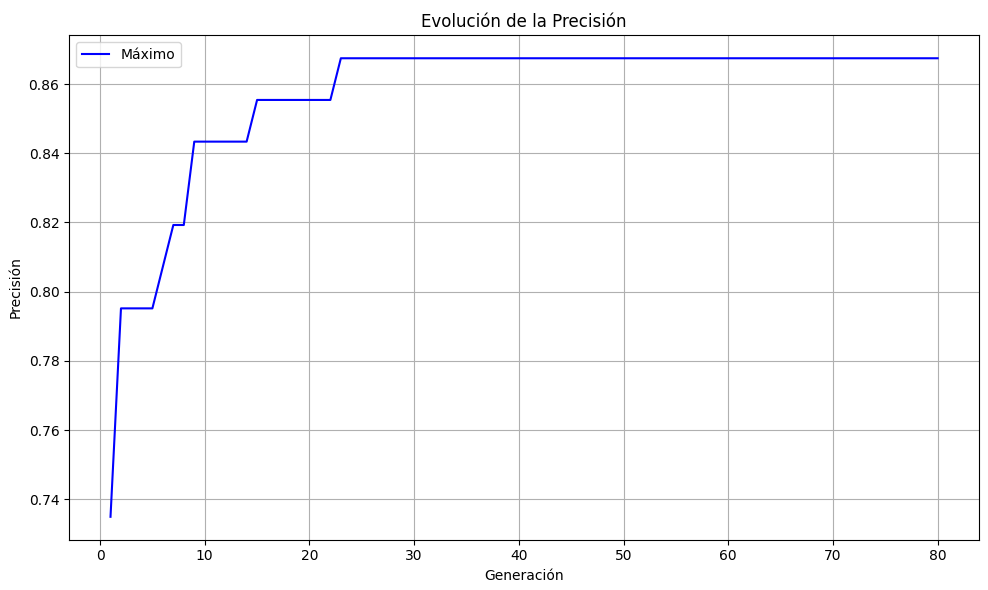
\includegraphics[width=1.0\textwidth]{plantilla-TFG-ETSIIT/doc/imagenes/Precision_gen.png}
    \caption{Gráfico algoritmo genético}
    \label{fig:etiqueta-imagen}
\end{figure}

Como se puede ver en el gráfico, el algoritmo evoluciona muy rápido, sin embargo, se estanca a partir de la generación 24. Los vectores que ha dado como resultado han sido los siguientes:

\begin{figure}[H]
    \centering
    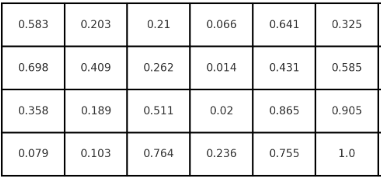
\includegraphics[width=1.0\textwidth]{plantilla-TFG-ETSIIT/doc/imagenes/Ataque_genetico.png}
    \caption{Vector de ataque genético}
    \label{fig:etiqueta-imagen}
\end{figure}

\begin{figure}[H]
    \centering
    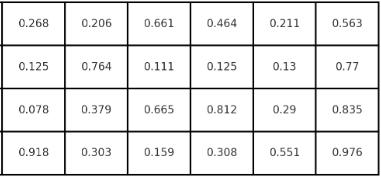
\includegraphics[width=1.0\textwidth]{plantilla-TFG-ETSIIT/doc/imagenes/Defensa_genetico.png}
    \caption{Vector de defensa genético}
    \label{fig:etiqueta-imagen}
\end{figure}

\section{Algoritmo genético con $\delta$}
Para intentar que la predicción sea lo más precisa posible, vamos ahora a añadir al vector de pesos a $\delta$, que es la variable que representa en qué momento cortar para decidir si gana uno, otro o hay empate. Hasta ahora esta variable había sido añadida a mano como 2, es decir si:

\begin{itemize}
    \item $Score global > 2$, gana local
    \item $Score global < -2$, gana visitante
    \item empate en caso contrario
\end{itemize}

Ahora el algoritmo genético, aparte de definir los vectores de ataque y defensa para las ponderaciones de las zonas del campo, también va a decidir esta variable. La configuración del algoritmo es igual a la que se ha explicado antes, excepto para la tasa de mutación, que al añadir un nuevo valor al vector ha pasado a ser de 1/49. El objetivo es comparar técnicas y ver cuál es más rentable en cuanto a precisión y recursos.

Los distintos valores con los que se va a probar son los mismos que antes, se ha ejecutado un total de 5 veces y se ha calculado la media de cada combinación y su desviación típica.

\begin{table}[H]
\centering
\caption{Resultados del algoritmo genético con $\delta $para diferentes configuraciones}
\label{tab:resultados_algoritmo}
\begin{tabular}{|c|c|c|c|c|c|}
\hline
\textbf{Población} & \textbf{Generaciones} & \textbf{Cruzamiento} & \textbf{Mutación} & \textbf{Precisión (\%)} & \textbf{ejecución (min)} \\
\hline
40 & 20 & 1 & 1/49 & $83.58 \pm 1.07$  & 13\\
40 & 20 & 0.9 & 1/49 & $83.6 \pm 1.03$ & 13 \\
40 & 40 & 0.9 & 1/49 & $83.58 \pm 0.65$ & 23 \\
40 & 40 & 1 & 1/49 & $85.02 \pm 1.37$ & 23 \\

80 & 20 & 0.9 & 1/49 & $85.5 \pm 1.47$ & 24\\
40 & 20 & 1 & 1/49 & $85.02 \pm 1.37$ & 24 \\
40 & 80 & 1 & 1/49 & $85.04 \pm 2.21$& 41 \\
40 & 80 & 0.9 & 1/49 & $84.78 \pm 1.37$ & 41 \\

80 & 40 & 0.9 & 1/49 & $86.22 \pm 0.65$ & 41\\
40 & 40 & 1 & 1/49 & $86.94 \pm 0.53$ & 41 \\
80 & 80 & 1 & 1/49 & $86.96 \pm 0.58$ & 86 \\
80 & 80 & 0.9 & 1/49 & $87.2 \pm 1.38$ & 86 \\

\hline
\end{tabular}
\end{table}

Como se puede apreciar, el mejor es el último con un 87.2 de precisión media y 1.38 de desviación típica. El gráfico al ejecutarlo es el siguiente:

\begin{figure}[H]
    \centering
    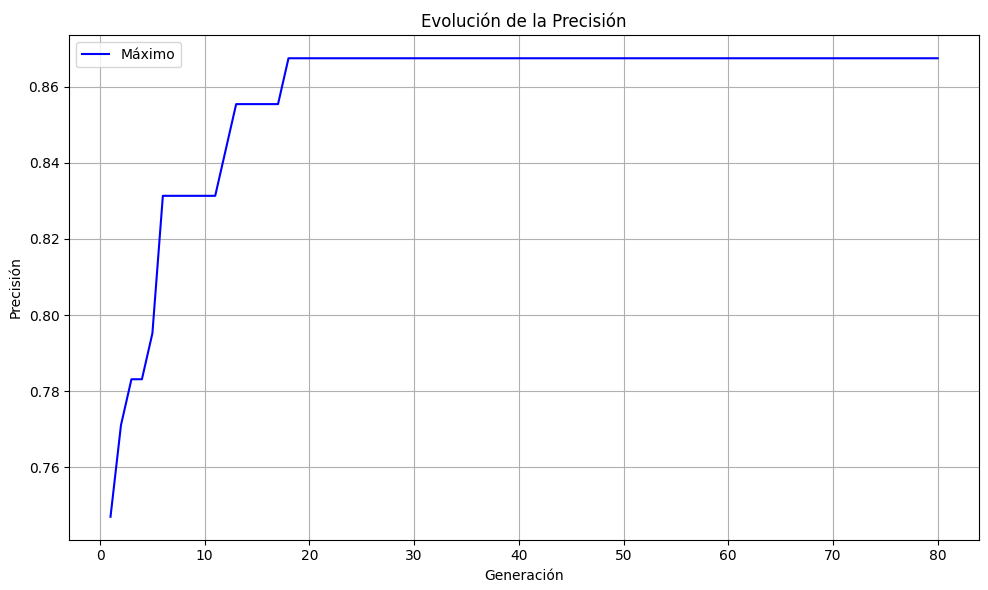
\includegraphics[width=1.0\textwidth]{plantilla-TFG-ETSIIT/doc/imagenes/Precision_delta.png}
    \caption{Grafico algoritmo genético}
    \label{fig:etiqueta-imagen}
\end{figure}

El gráfico es muy parecido al anterior, empieza evolucionando rápido, sin embargo, a partir de la generación 18 se estanca y no consigue avanzar más. Los vectores resultado son:

\begin{figure}[H]
    \centering
    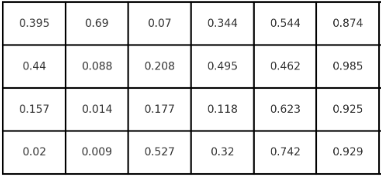
\includegraphics[width=1.0\textwidth]{plantilla-TFG-ETSIIT/doc/imagenes/Ataque_gen_delta.png}
    \caption{Vector de ataque genético con $\delta$}
    \label{fig:etiqueta-imagen}
\end{figure}

\begin{figure}[H]
    \centering
    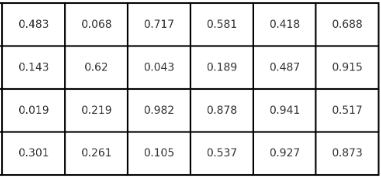
\includegraphics[width=1.0\textwidth]{plantilla-TFG-ETSIIT/doc/imagenes/Defensa_gen_delta.png}
    \caption{Vector de defensa genético con $\delta$}
    \label{fig:etiqueta-imagen}
\end{figure}

\section{Conclusión}
Realmente no hay mucha diferencia entre un algoritmo y otro, por lo que se puede llegar a la conclusión de que el punto en el que decidir cortar el score global para definir el ganador no es determinante, seguramente porque cada partido tenga unos valores más grandes o pequeños según su desarrollo, y la puntuación de los equipos se adaptan a las circunstancias, por lo que los partidos no siguen una tendencia fija de score global.

A parte de eso, el porcentaje de acierto que se puede llegar a alcanzar ($87.2 \pm 1.38$) es bastante elevado para un partido de fútbol, por lo que se puede decir de manera satisfactoria que se ha cumplido el objetivo inicial de este TFG.
